\documentclass[
%% TIKZ_CLASSOPTION %%
tikz
]{standalone}
\usepackage{amsmath}
\usetikzlibrary{matrix}
%% EXTRA_TIKZ_PREAMBLE_CODE %%
\begin{document}
%% TIKZ_CODE %%
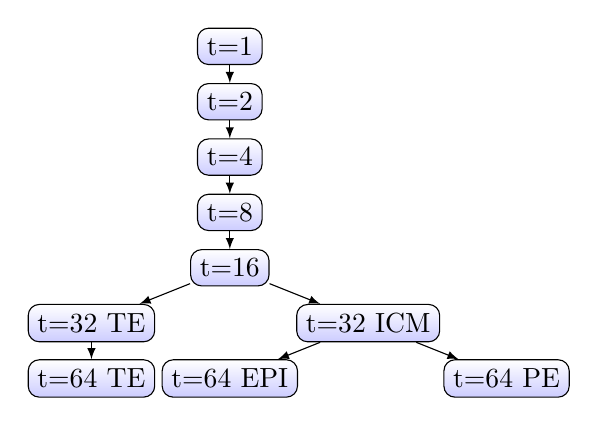
\begin{tikzpicture}[sibling distance=10em, level distance=2em,
  every node/.style = {shape=rectangle, rounded corners,
    draw, align=center, top color=white, bottom color=blue!20},
    edge from parent/.style={draw, -latex}]

% Define the tree structure
\node {t=1}
    child { node {t=2}
        child { node {t=4}
            child { node {t=8}
                child { node {t=16}
                    child { node {t=32 TE}
                        child { node {t=64 TE} }
                    }
                    child { node {t=32 ICM}
                        child { node {t=64 EPI} }
                        child { node {t=64 PE} }
                    }
                }
            }
        }
    };
\end{tikzpicture}
\end{document}
